\chapter[Strucuture of Crystals and Liquids]{Ground State Structures of Molecular Crystals and Liquids}
\label{sec:structure}

As we lower the temperature, the properties of a condensed phase become increasingly dominated by the arrangement of molecules corresponding to the local potential energy minima, the ground state. In the same way the structure and dynamics of a small molecule can be inferred from its ground state structure, these properties can be inferred from the ground state of these condensed phases with thousands of molecules.

In this chapter we address: What are the structures and energies of the most stable crystal structures of our molecules? The problems with generic measures of order in molecular systems? What degree of ordering is present in the ground states of our molecular liquids?

\section{The Most Stable Crystal Phase}

The most stable crystal phase, for our purposes, is the crystal that will form spontaneously from the liquid phase upon cooling. Since by design this process is slow or unobservable for the molecular liquids we are using we need to use other means to identify the most stable crystal phase (described below). Of most stable crystal phases~\figref{crystals} the \dcon and \tri molecules have unit cells in the p2 wallpaper group in which the majority of crystals lie~\cite{plass:07,jennings:15}. While the \done molecule is contained in the p2mg wallpaper group which contains very few crystal structures, making it an interesting crystal structure.

\begin{figure}
    \centering
    \begin{subfigure}[t]{0.45\linewidth}
        \includegraphics[width=\textwidth]{{{Snowman-0.4-0.637556-1.00-p2mg-frame}}}
        \caption{}
        \label{fig:crystal done}
    \end{subfigure}\hfill
    \begin{subfigure}[t]{0.45\linewidth}%
        \includegraphics[width=\textwidth]{{{Snowman-0.4-0.637556-1.637556-p2-frame}}}
        \caption{}
        \label{fig:crystal dcon}
    \end{subfigure}
    \begin{subfigure}{0.45\linewidth}
        \includegraphics[width=\textwidth]{{{Trimer-0.4-0.637556-1.00-120-p2-frame}}}
        \caption{}
        \label{fig:crystal tri}
    \end{subfigure}
    \caption{The stable crystal forms of the \done~\subfigref{crystal done}, \dcon~\subfigref{crystal dcon}, and \tri~\subfigref{crystal tri} phases for each molecule. The molecules are coloured according to their orientation. The unit cell is indicated by a black box with an inversion center marked with a red dot.}
    \label{fig:crystals}
\end{figure}

The crystal structures shown in \textfigref{crystals} were determined to be the most stable crystal structures using a variety of techniques. As a starting point we wanted to find the lowest energy crystal structures, since using molecular dynamics was not possible we had to use an alternate method. By approximating our particles as hard discs and finding the closest packed structure we are able to use the isopointal search algorithm developed by~\textcite{husdon:10} to search the reduced packing space, generating a best packed structure for each wallpaper group.

The best packed structures can then be used as the starting configurations for a molecular dynamics simulation to find the lowest energy ground state~\tabref{crystal energies}. The \done and \dcon molecules have configurations with a ground state significantly lower than any other, p2mg and p2 respectively. For these two molecules we can be fairly certain these are the most stable ground state, however for the \tri molecule there are three configurations p2, p2gg and pg all with similar ground state energies.

 
\begin{table}
    \sisetup{
        table-format = +3.4,
        table-omit-exponent,
        fixed-exponent =-4,
        parse-numbers=true,
        scientific-notation=true,
        round-mode=places,
        round-precision=3}
    \centering
    \begin{tabular}{ | l | S  S  S | }
        \hline
        {Crystal} & \multicolumn{3}{c|}{Energy per molecule (\num{e-4})} \\
            &\done & \dcon & \tri \\ \hline
        p2 & 0.00001376280055& {\cellcolor{blue!20}}0.0001527208398& {\cellcolor{blue!10}}-0.0003934685913\\
        p2mg & {\cellcolor{blue!20}}0.000005732595806& 0.0004479052484& -0.0003354198174\\
        p2gg & 0.00002632511042& 0.0001699363766& {\cellcolor{blue!20}}-0.000401823091\\
        pg & 0.00002824743917& 0.0002860863393& {\cellcolor{blue!10}}-0.0004000561542\\
        p3 & 0.00003468842645& 0.0002424453316& -0.0003292839541\\
        \hline
    \end{tabular}
    \caption{The energy per molecule for a variety of the best packing crystal structures. Both the \done and \dcon systems have an arrangement with significantly lower energy, p2mg and p2 respectively. While the \tri system has three arrangements with very similar energies, the p2, p2gg and pg wallpaper groups.}
    \label{tab:crystal energies}
\end{table}

With multiple structures of the \tri molecule having similar energies further analysis is required to determine the most stable structure, for this we looked to a two phase system as described in \textsecref{two phase}. The two phase system~\figref{tri two phase} showed a rearrangement of molecules from the p2gg structure, which had the lowest ground state energy, to the p2 structure. The most likely reason for this phase transition from p2gg structure is an increased entropy in the p2 structure, hence thermodynamic stability at higher temperatures. From this analysis the p2 structure was considered the most stable structure.


\begin{figure}
    \begin{subfigure}[t]{0.5\textwidth}
        \includegraphics[width=\textwidth]{{{Trimer-1.30-0.637556-1.00-120-p2gg-1-frame-0000000000}}}
        \caption{Initial}
        \label{fig:tri rearr init}
    \end{subfigure}
    \begin{subfigure}[t]{0.5\textwidth}
        \includegraphics[width=\textwidth]{{{Trimer-1.30-0.637556-1.00-120-p2gg-1-frame-0320000000}}}
        \caption{Final}
        \label{fig:tri rearr fine}
    \end{subfigure}
    \caption{The initial~\subfigref{tri rearr init} and final~\subfigref{tri rearr fine} configurations of a two phase simulation of the \tri molecule below the melting point. We can see the solid state phase transition from a p2mg structure with four layers in each unit cell to a structure that alternates between the p2 structure (two layers) and the p2gg structure (4 layers).}
    \label{fig:tri two phase}
\end{figure}

In light of the \tri molecule having a stable structure that did not have the lowest energy ground state we performed melting point analysis on the \done and \dcon molecules. The melting points for each crystal were obtained using a two phase system~\tabref{melting}. These results confirmed the lowest energy structures were the most stable having significantly higher melting points.

\begin{table}
    \centering
    \begin{tabular}{| l l | S |}
        \hline
        Molecule & Crystal & {Melting Point} \\ \hline
        \multirow{3}{*}{\done} & p2 & 0.65 \\
                               & p2gg & 0.55 \\
                               & p2mg & 0.92 \\ \hline
        \multirow{2}{*}{\dcon} & p2 & 1.85 \\
                               & p2gg & 1.50 \\ \hline
    \end{tabular}
    \caption{Melting points of the crystal phases established from two phase systems.}
    \label{tab:melting}
\end{table}

\section{Quantifying Order in Molecular Systems}

In most cases it is fairly easy to distinguish a crystal from an amorphous phase by simple visual inspection of the two configurations. Much harder to determine visually is to quantify the degree to which a system is ordered, a problem with application in crystal growth. In this section we investigate a number of measures of order, including local order, as well as problems associated with each. We will be investigating these order parameters using an amorphous and crystal configuration~\figref{frame comp} of the \dcon molecule.

\begin{figure}
    \begin{subfigure}{0.5\textwidth}
        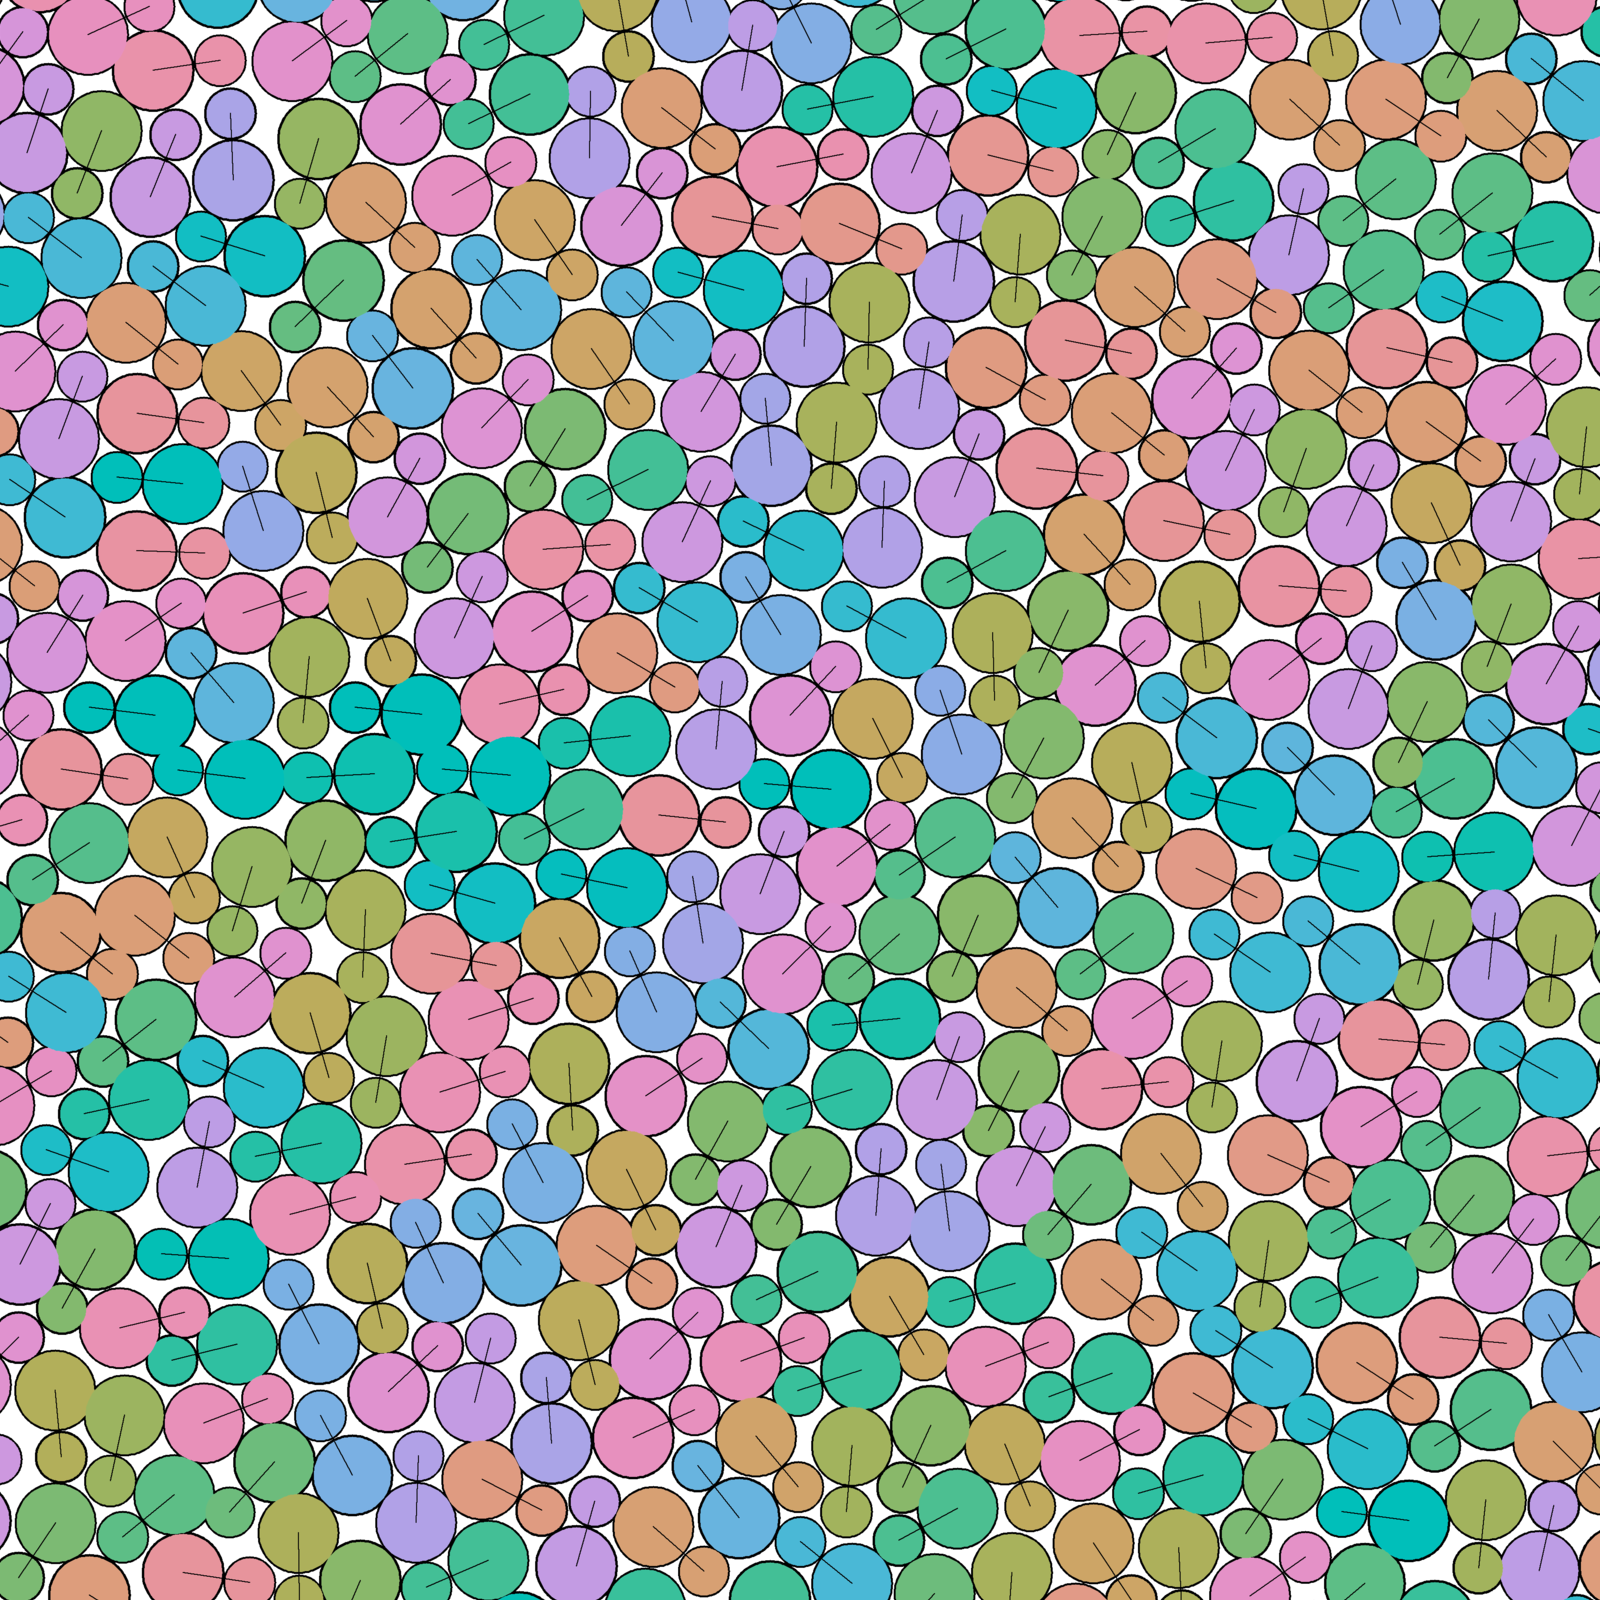
\includegraphics[width=\linewidth]{amorphous-frame}
        \caption{}
        \label{fig:amorphous frame}
    \end{subfigure}
    \begin{subfigure}{0.5\textwidth}
        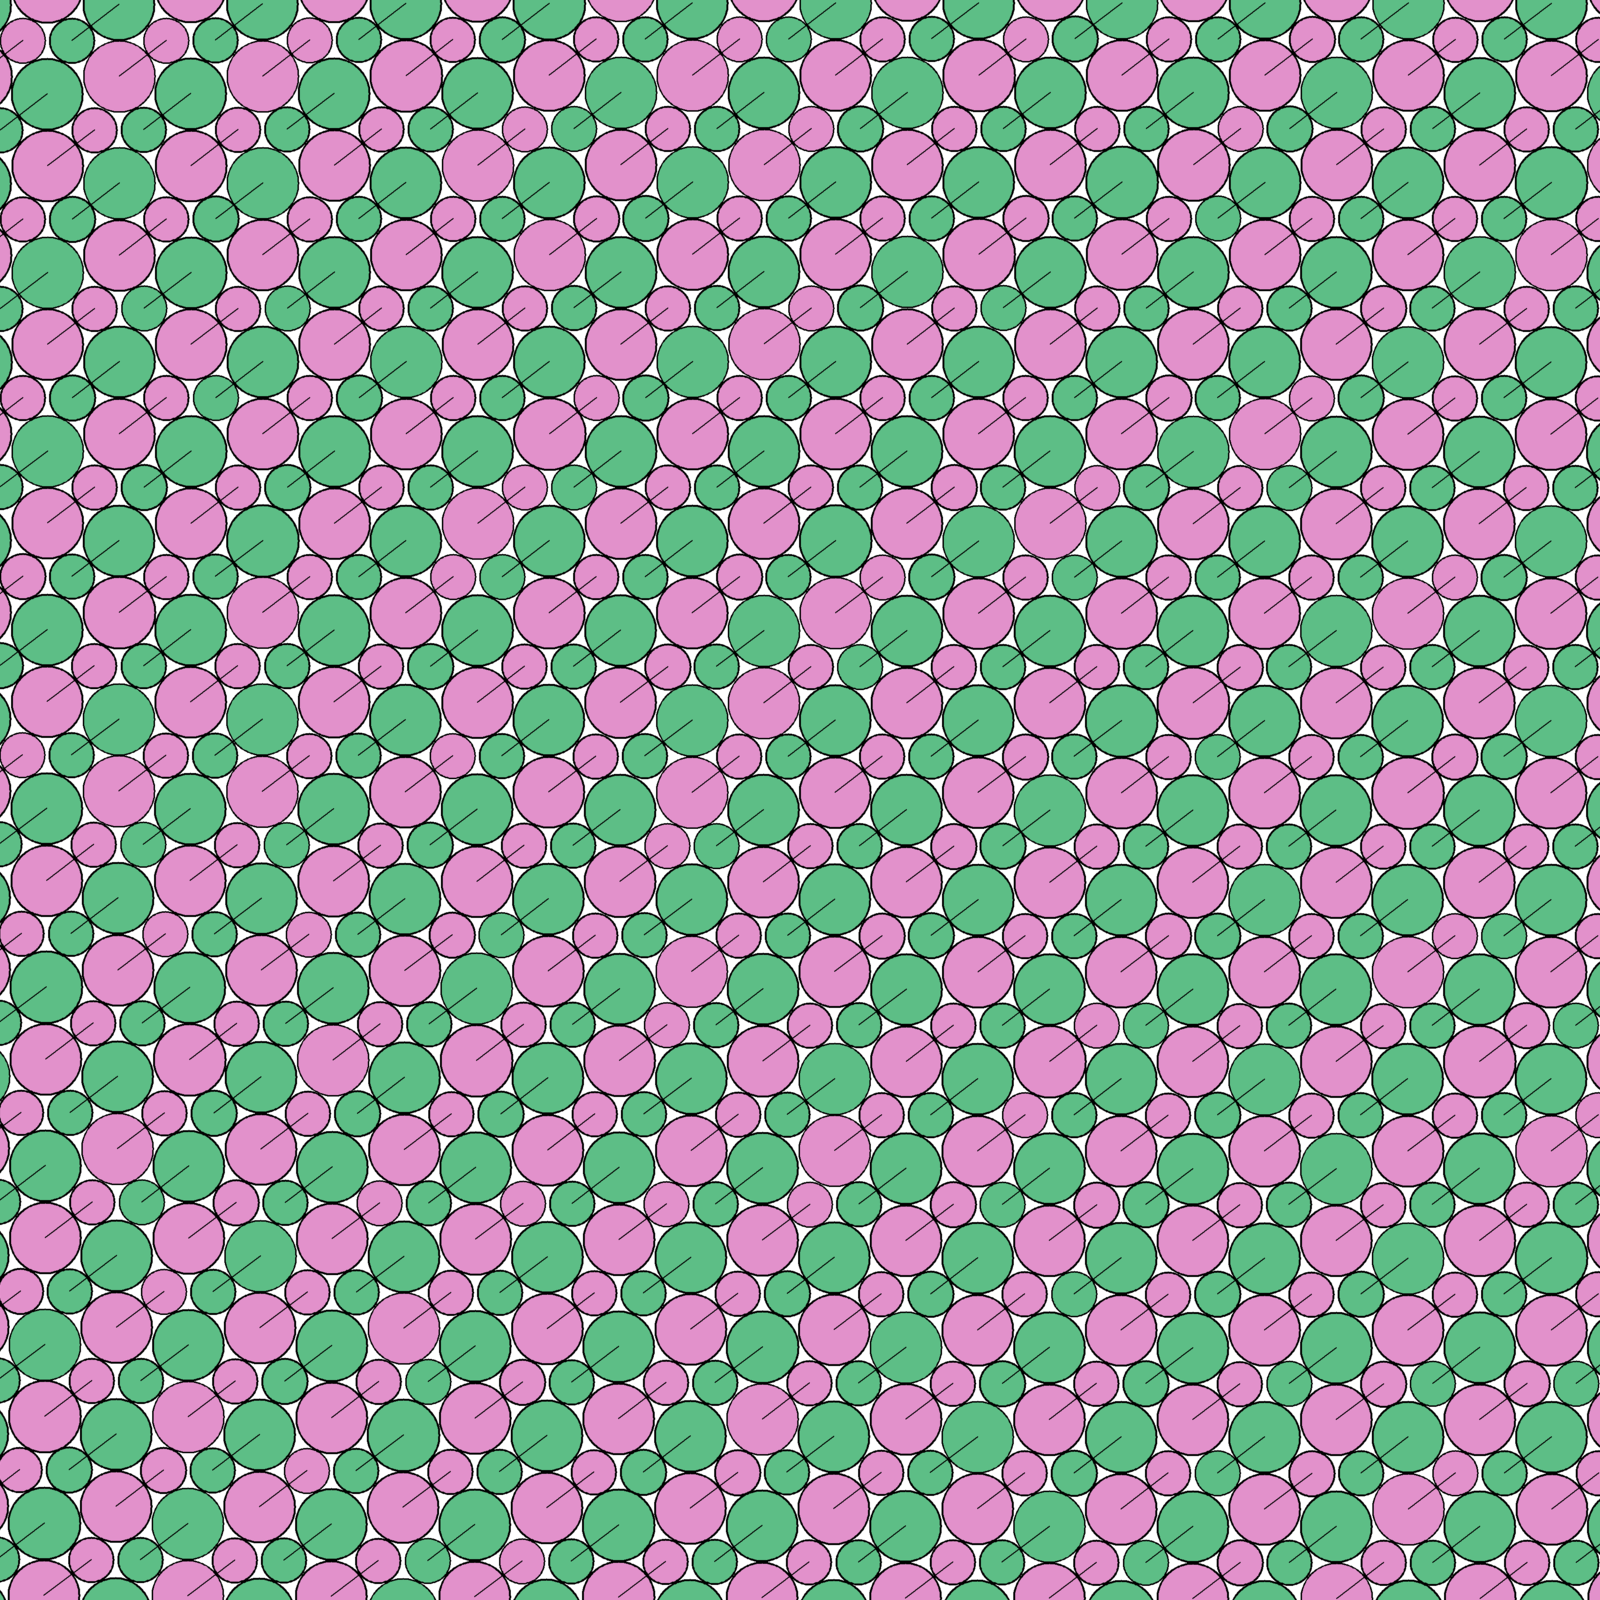
\includegraphics[width=\linewidth]{crys-frame}
        \caption{}
        \label{fig:crys frame}
    \end{subfigure}
    \caption{The amorphous \subfigref{amorphous frame} and crystal \subfigref{crys frame} configurations with the colour of the molecules indicating orientation.}
    \label{fig:frame comp}
\end{figure}

The first of the order parameters is the radial distribution function~\figref{radial comp}, a distribution of the relative intermolecular distances. The amorphous structure shows short range ordering characteristic of any condensed phase, however this order is only present in the first layer of molecules, once past this region the distribution of molecules is uniform. This is in contrast with the crystal structure that exhibits distinct peaks out to long ranges showing the long range order of this structure.

\begin{figure}
    \begin{subfigure}{0.5\textwidth}
        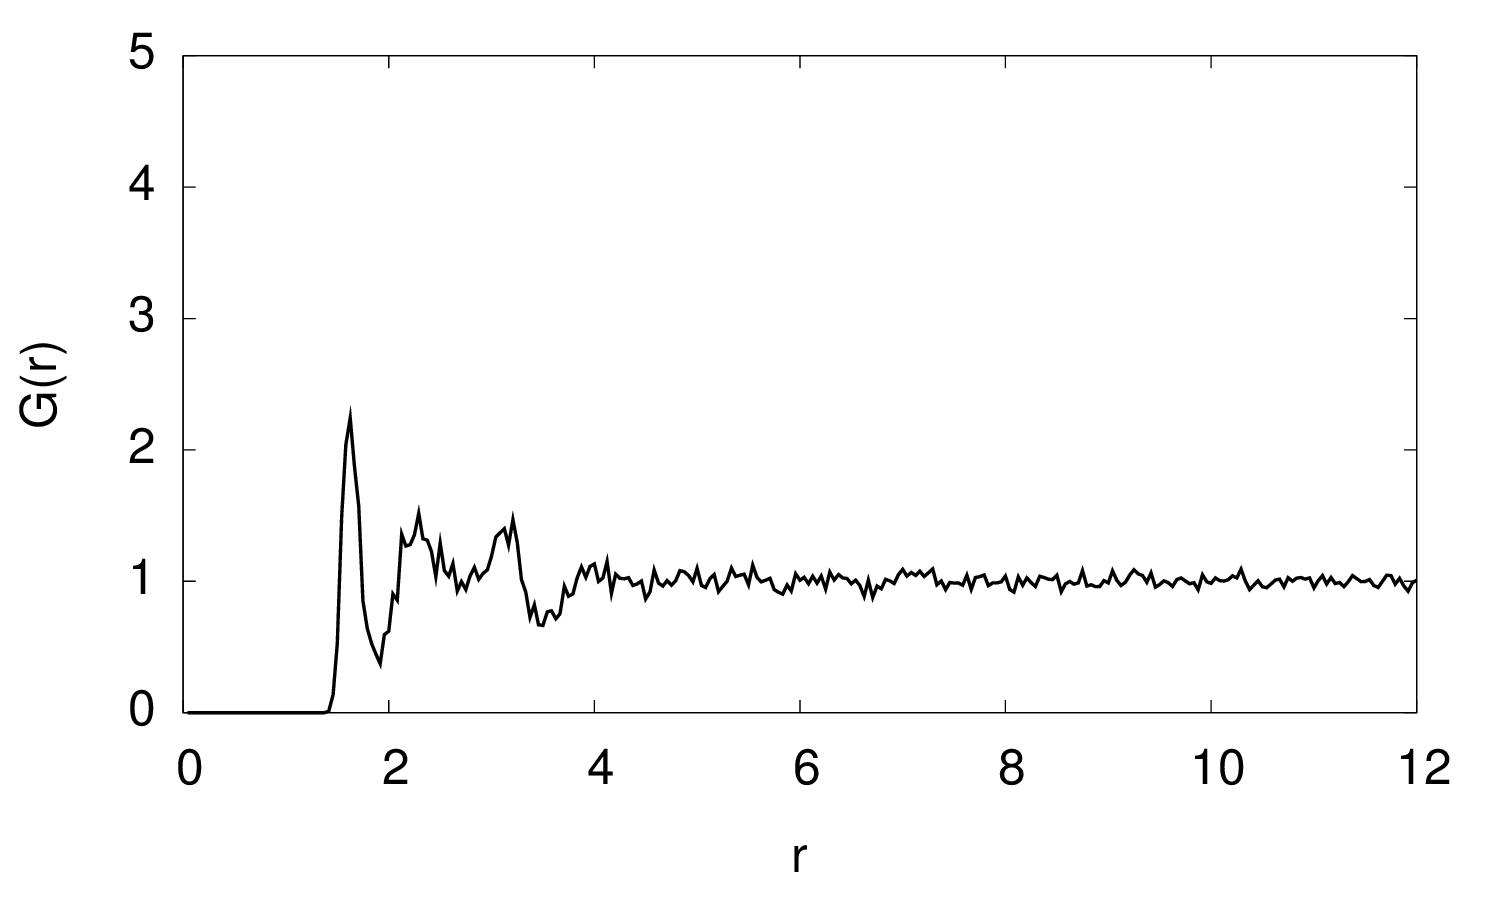
\includegraphics[width=\linewidth]{amorphous-radial}
        \caption{}
        \label{fig:amorphous radial}
    \end{subfigure}
    \begin{subfigure}{0.5\textwidth}
        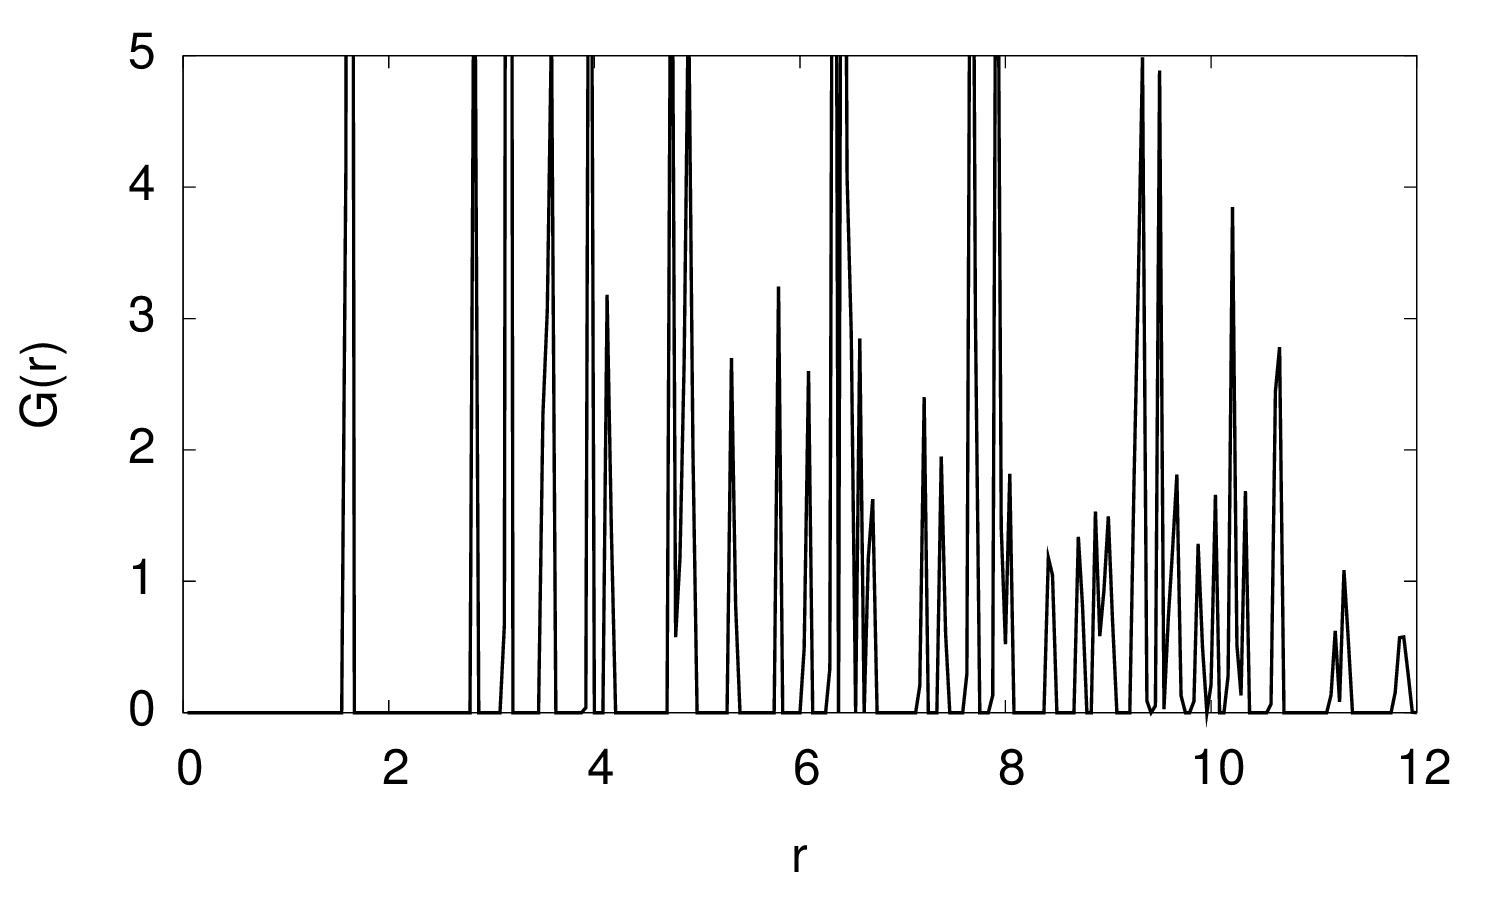
\includegraphics[width=\linewidth]{crys-radial}
        \caption{}
        \label{fig:crys radial}
    \end{subfigure}
    \caption{The amorphous \subfigref{amorphous radial} and crystal \subfigref{crys radial} radial distribution functions. The amorphous structure shows a peak at short range which quickly becomes a uniform distribution. The crystal structure shows sharp peaks out to long ranges.}
    \label{fig:frame comp}
\end{figure}

Along with the global order measured by the radial distribution function we can also measure local order to classify molecules as crystalline or amorphous. This allows a count of the number of molecules that are considered crystalline, an easy measure of crystal growth. The crystal structures of all three molecules have the molecules aligned antiparallel to each other, all molecules are either \ang{0} or \ang{180} relative to each other. We can use this to define a local order parameter $O_\text{local}$,
\begin{equation}
    O_{\text{local}} = \frac{1}{N_{\text{neigh}}}\sum_{i=1}^{N_\text{neigh}} (\vect{\hat e} \cdot \vect{\hat e_i})^2
\end{equation}
where $N_\text{neigh}$ is the number of neighbours, $\vect{\hat e}$ is the unit orientation vector of the molecule and $\vect{\hat e_i}$ is the unit orientation vector of each neighbour. In the perfect crystal structure molecules with $O_\text{local}=1$ would be considered crystalline, however to account for the rotations and vibrations of molecules when heated up a cutoff of \num{0.8} was chosen as being best at differentiating crystal $O_\text{local}> 0.8$ and amorphous $O_\text{local} < 0.8$ regions. To assist in identifying this local order within a configuration~\figref{local comp} we can colour the ordered molecules leaving all others grey. Since this local order parameter identifies molecules with antiparallel orientations the molecules are coloured such that both have the same colour. The coloured regions of the amorphous phase show molecules or small clusters that exhibit short range ordering, with the number of local orderings in the amorphous phase some are going to be considered locally crystalline.

\begin{figure}
    \begin{subfigure}{0.5\textwidth}
        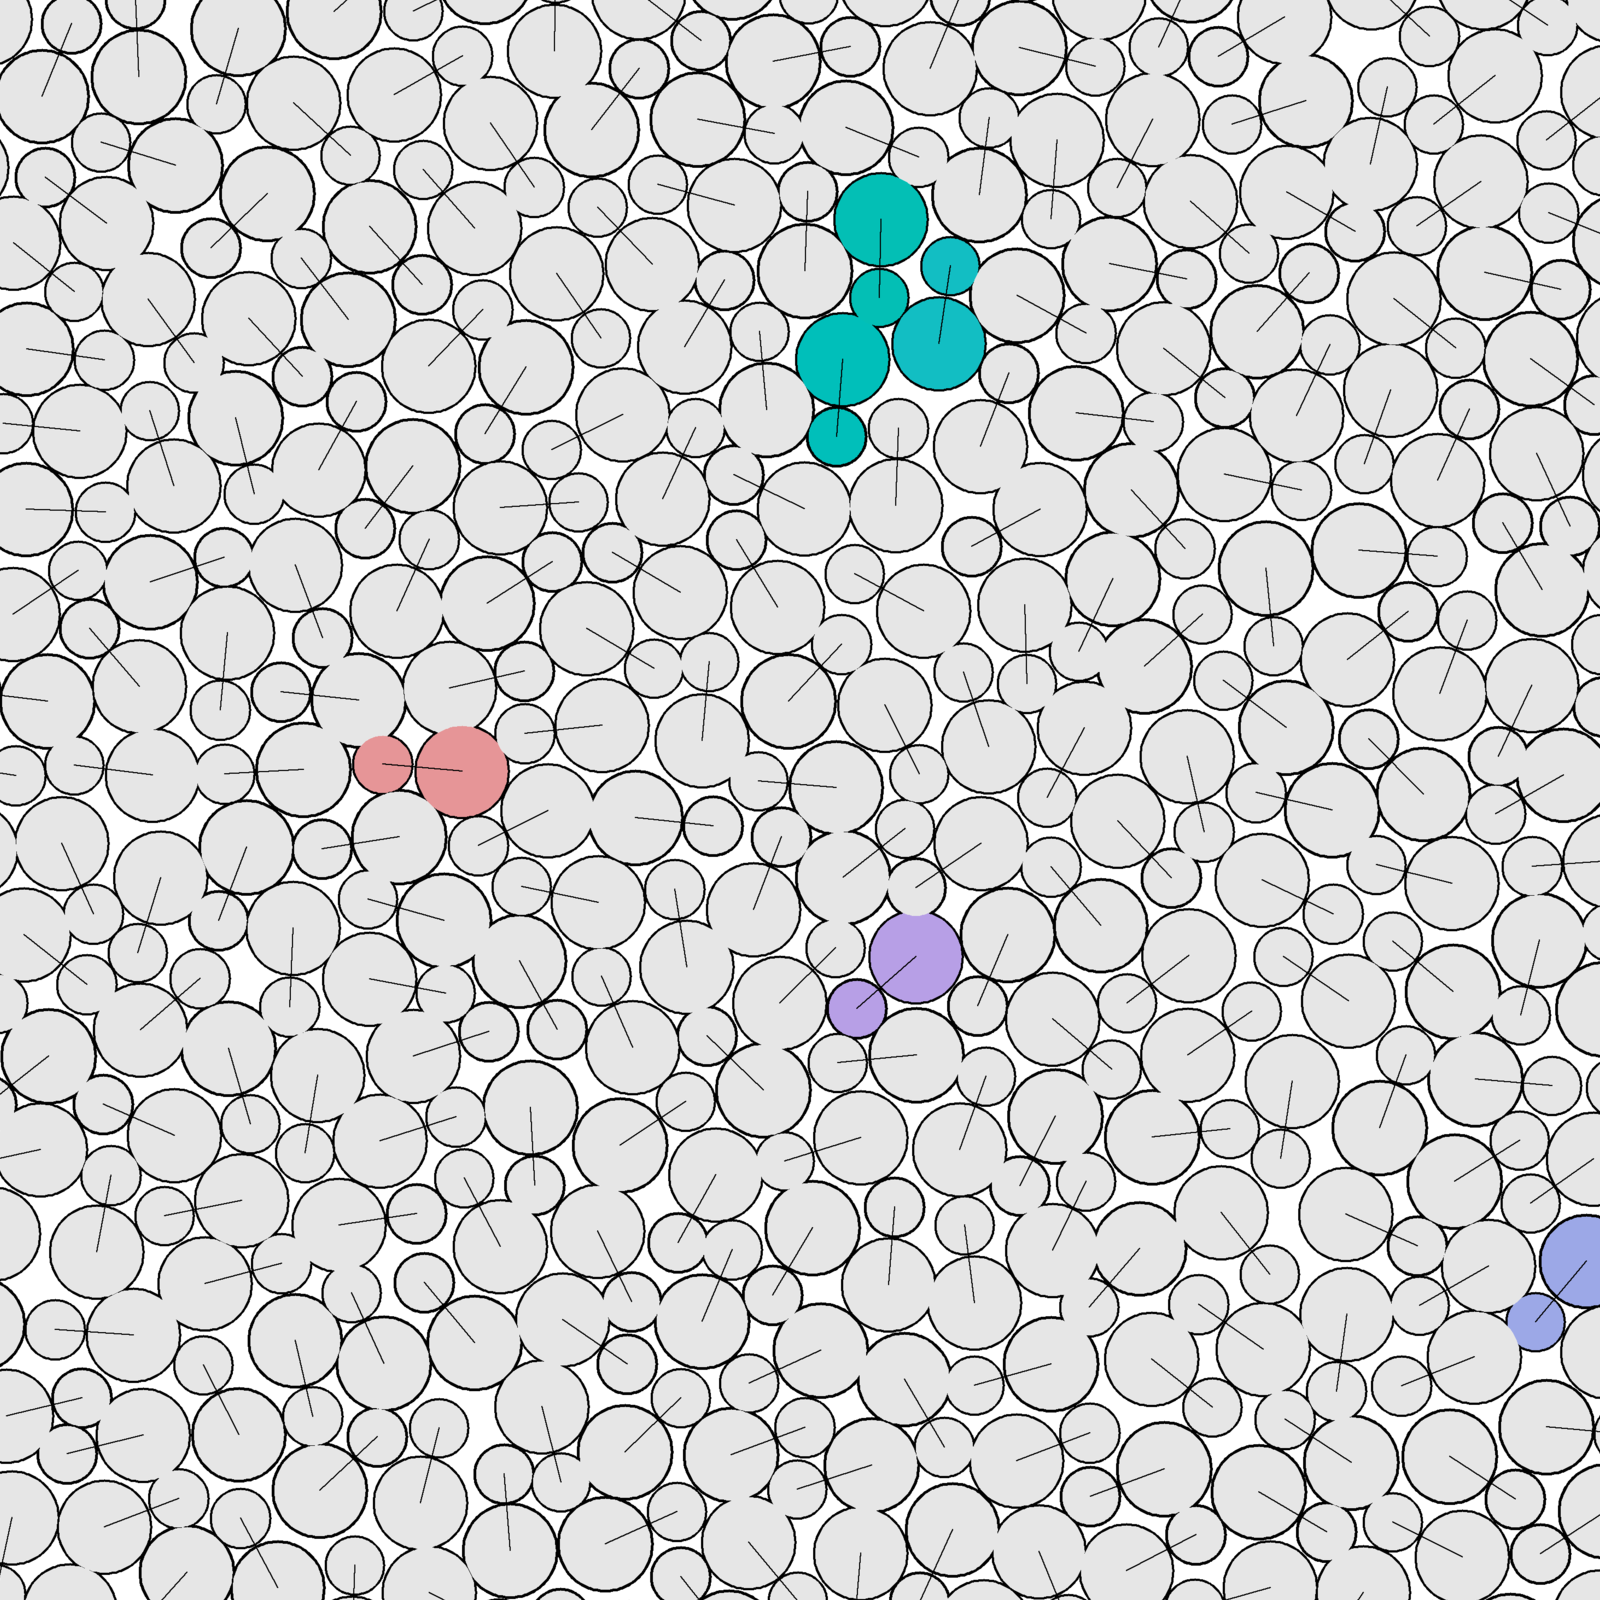
\includegraphics[width=\linewidth]{amorphous-local}
        \caption{}
        \label{fig:amorphous radial}
    \end{subfigure}
    \begin{subfigure}{0.5\textwidth}
        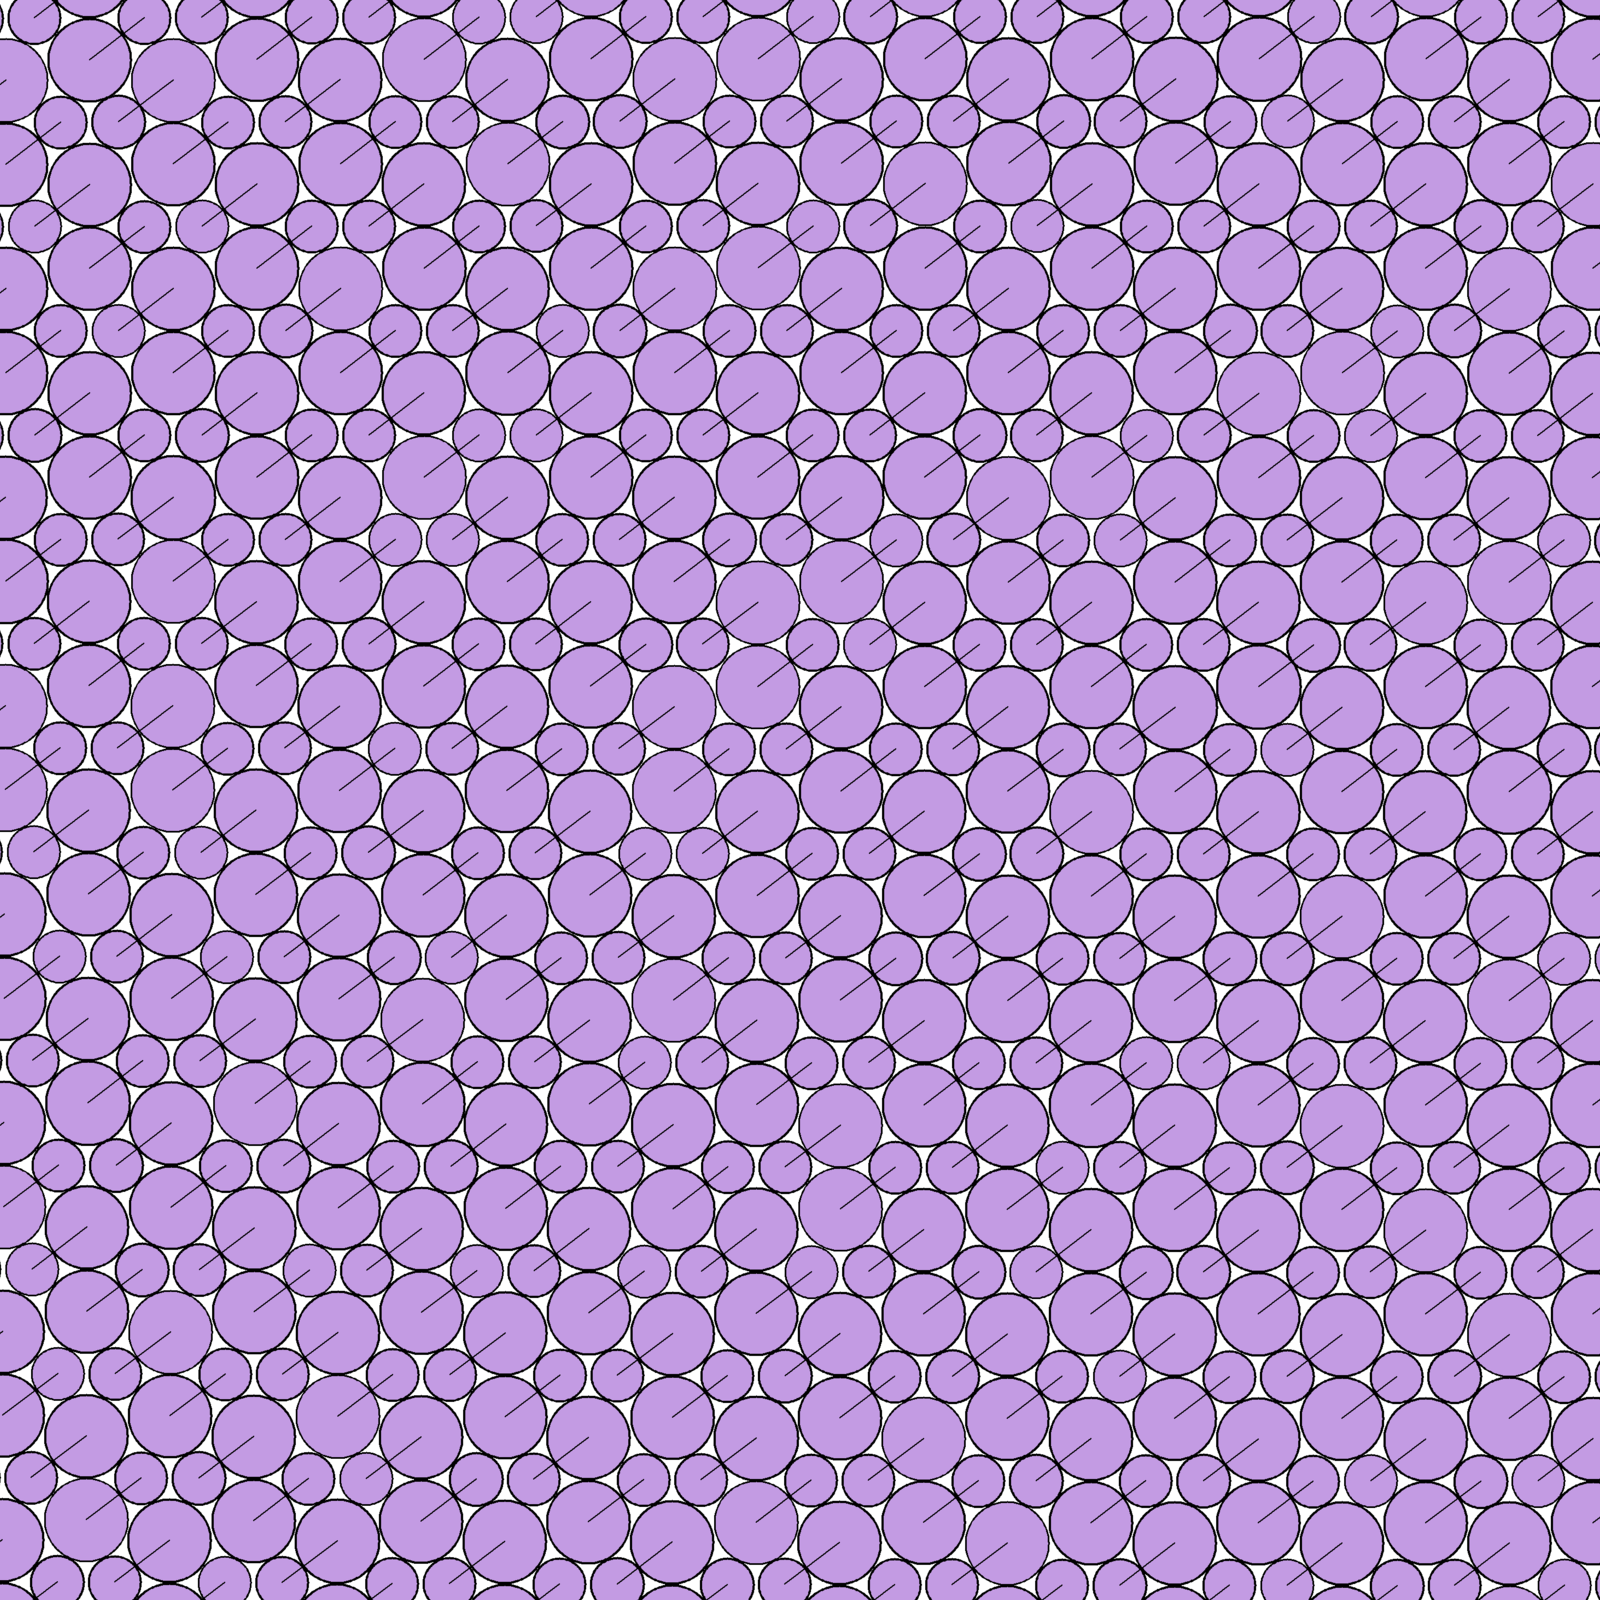
\includegraphics[width=\linewidth]{crys-local}
        \caption{}
        \label{fig:crys radial}
    \end{subfigure}
    \caption{The amorphous \subfigref{amorphous local} and crystal \subfigref{crys local} configurations with the colouring identifying local order. The molecules are coloured according to the orientation of the crystal. The crystal phase shows a single purple crystal for the entire configuration, while the amorphous phase has a few individual molecules showing order with a small cluster.}
    \label{fig:frame comp}
\end{figure}

\subsection{Problems with Generic Descriptions of Order in Molecular Systems}

The \dcon molecule was chosen for being a special case, this ratio of hard discs will form a compact packing~\appref{compact packing}. If we start with the compact packing of discs~\figref{compact} we can assign bonds between large and small particles to form molecules without modifying the underlying structure. Two examples of this assignment of bonds, an orientationally ordered p2 structure~\figref{ordered-frame} and an orientationally disordered random assignment of bonds~\figref{random-frame}. Both these structures have the same underlying structure of particles, despite the orientational disorder in the randomly assigned configuration it is indisputably crystalline in character and any order parameter should reflect this.

\begin{figure}
    \centering
    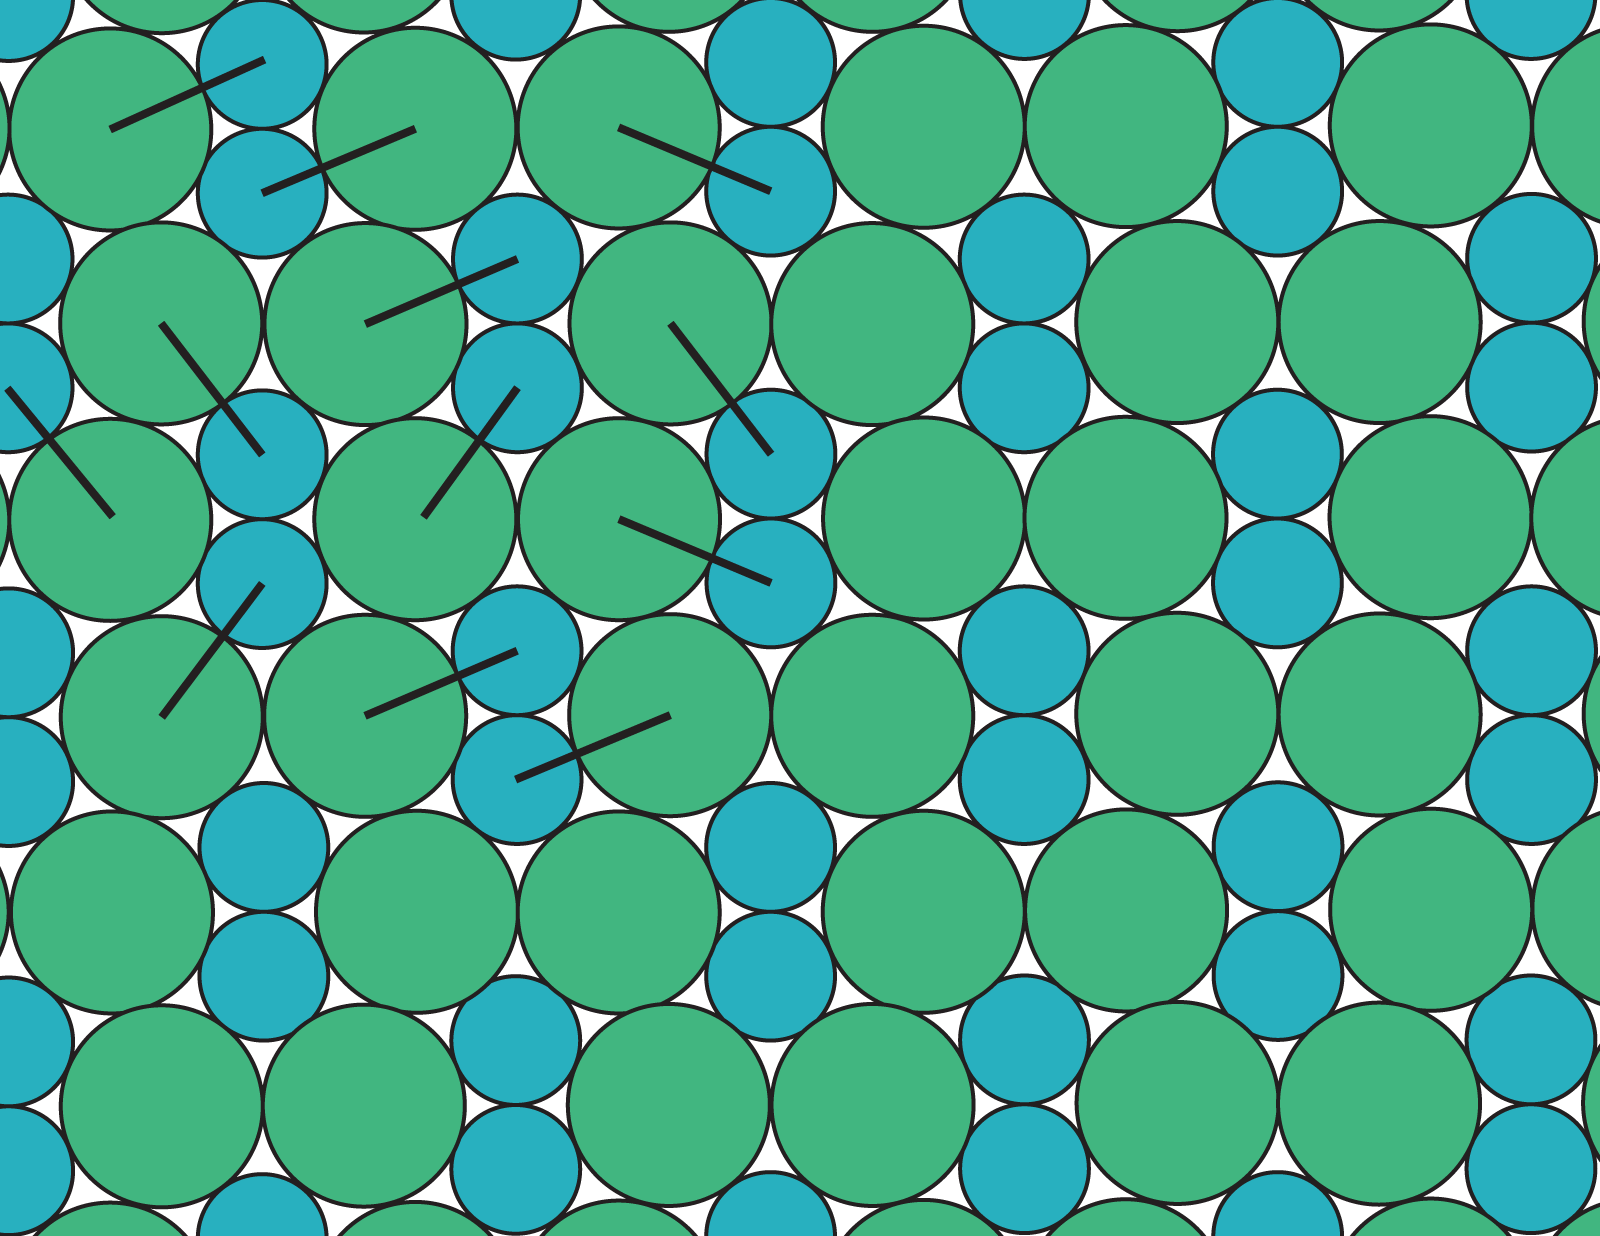
\includegraphics[width=0.5\textwidth]{compact}
    \caption{The compact packing of discs with ratio 1:0.637556. Assignment of bonds to this structure can be performed randomly (top left) with no alteration of the underlying structure.}
    \label{fig:compact}
\end{figure}

Using the local order parameter~\figref{compact local} the orientationally ordered configuration has the expected crystal structure while the orientationally disordered structure is not considered crystalline. For the \dcon molecule the more complex and specific crystal phase makes a general order parameter insufficient to resolve the crystal structure. Instead we want a local order parameter designed specifically for the \dcon system.

\begin{figure}
    \begin{subfigure}[t]{0.5\linewidth}
        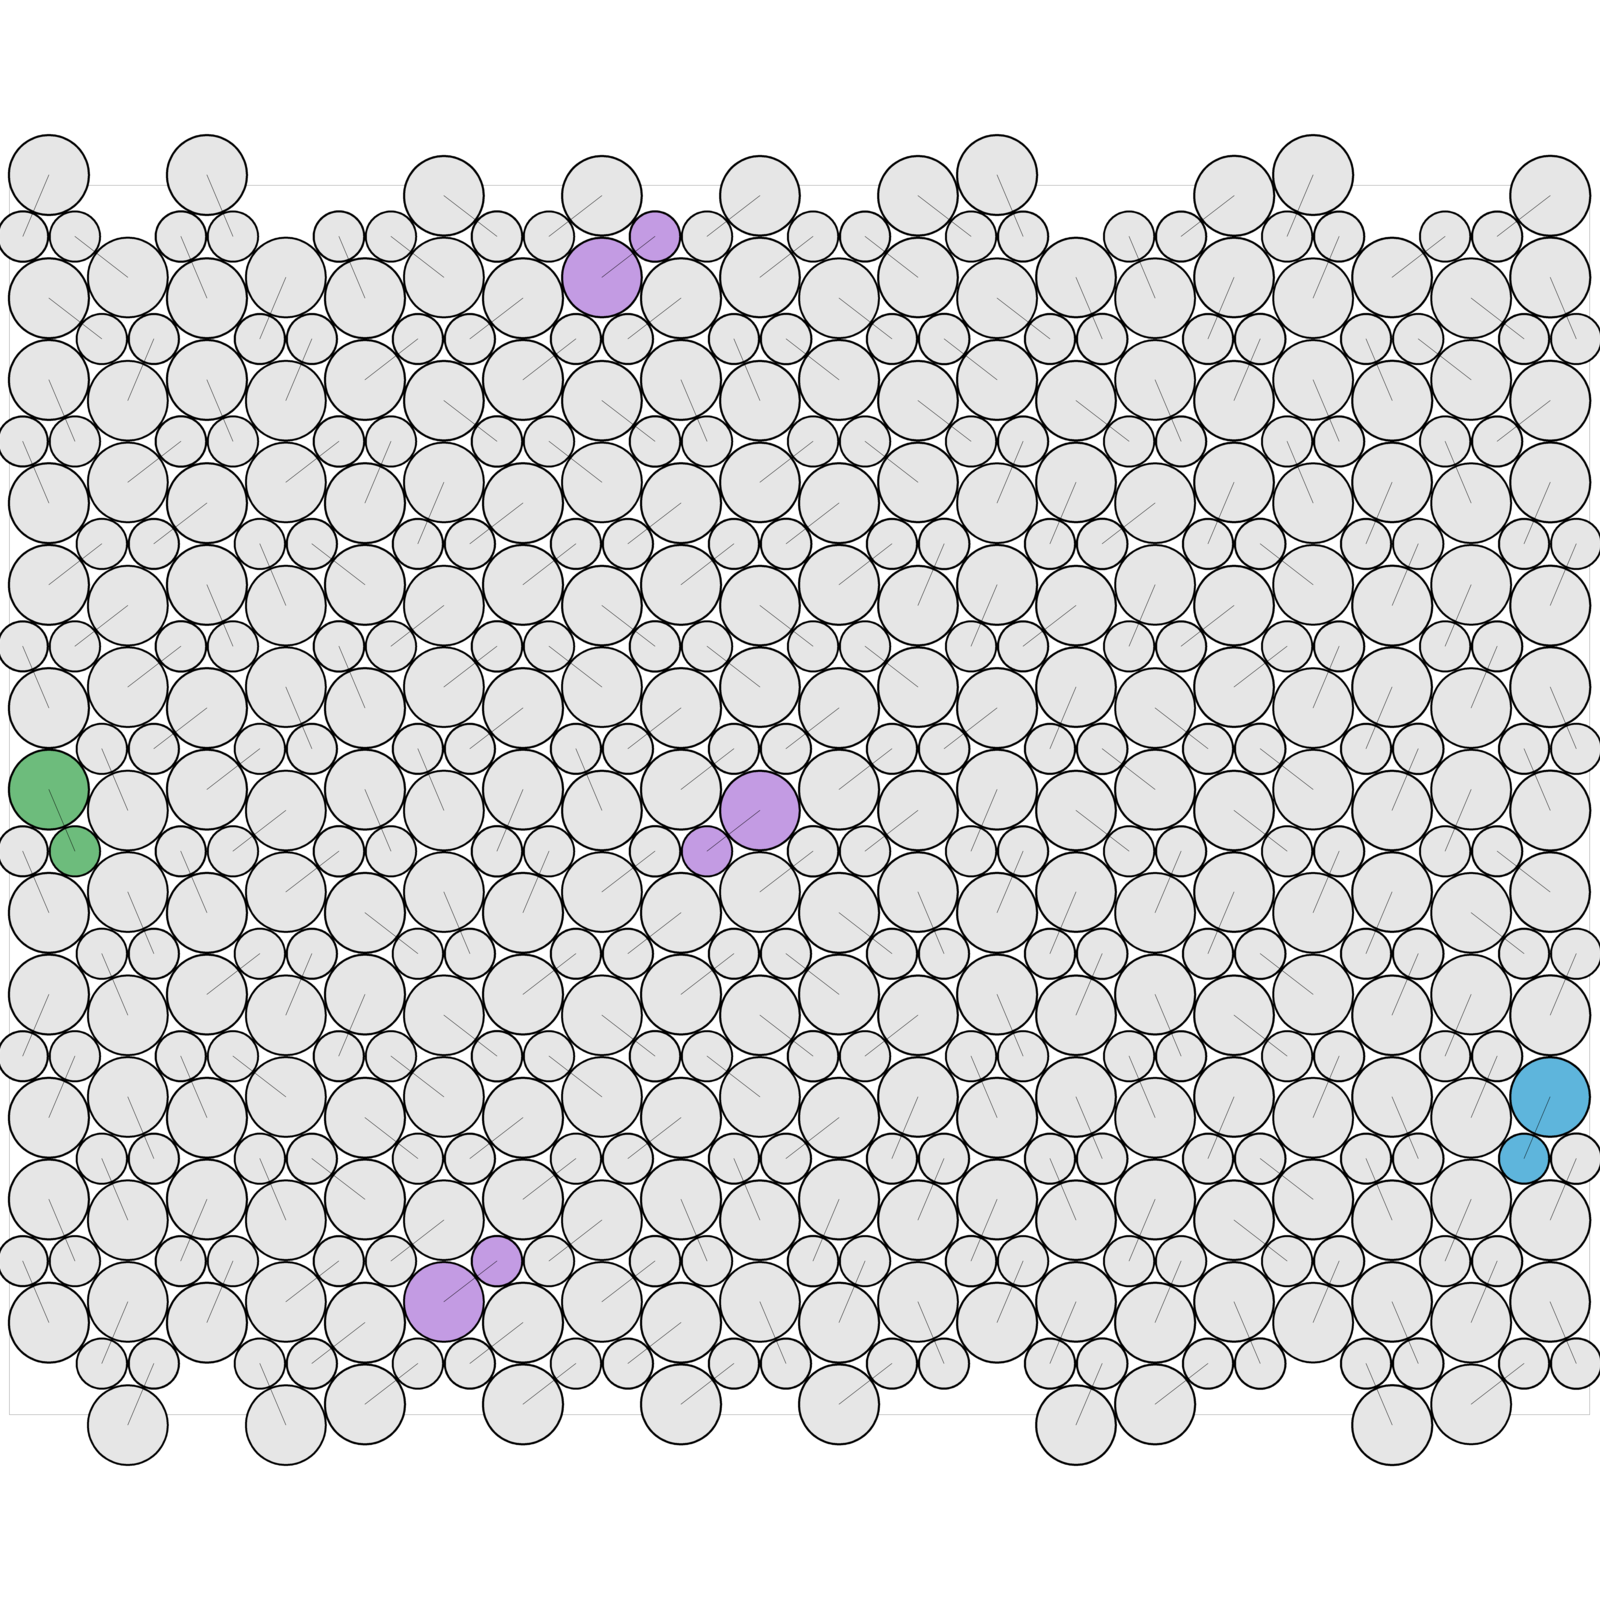
\includegraphics[width=\linewidth]{random-local}
        \caption{}
        \label{fig:random local}
    \end{subfigure}
    \begin{subfigure}[t]{0.5\linewidth}
        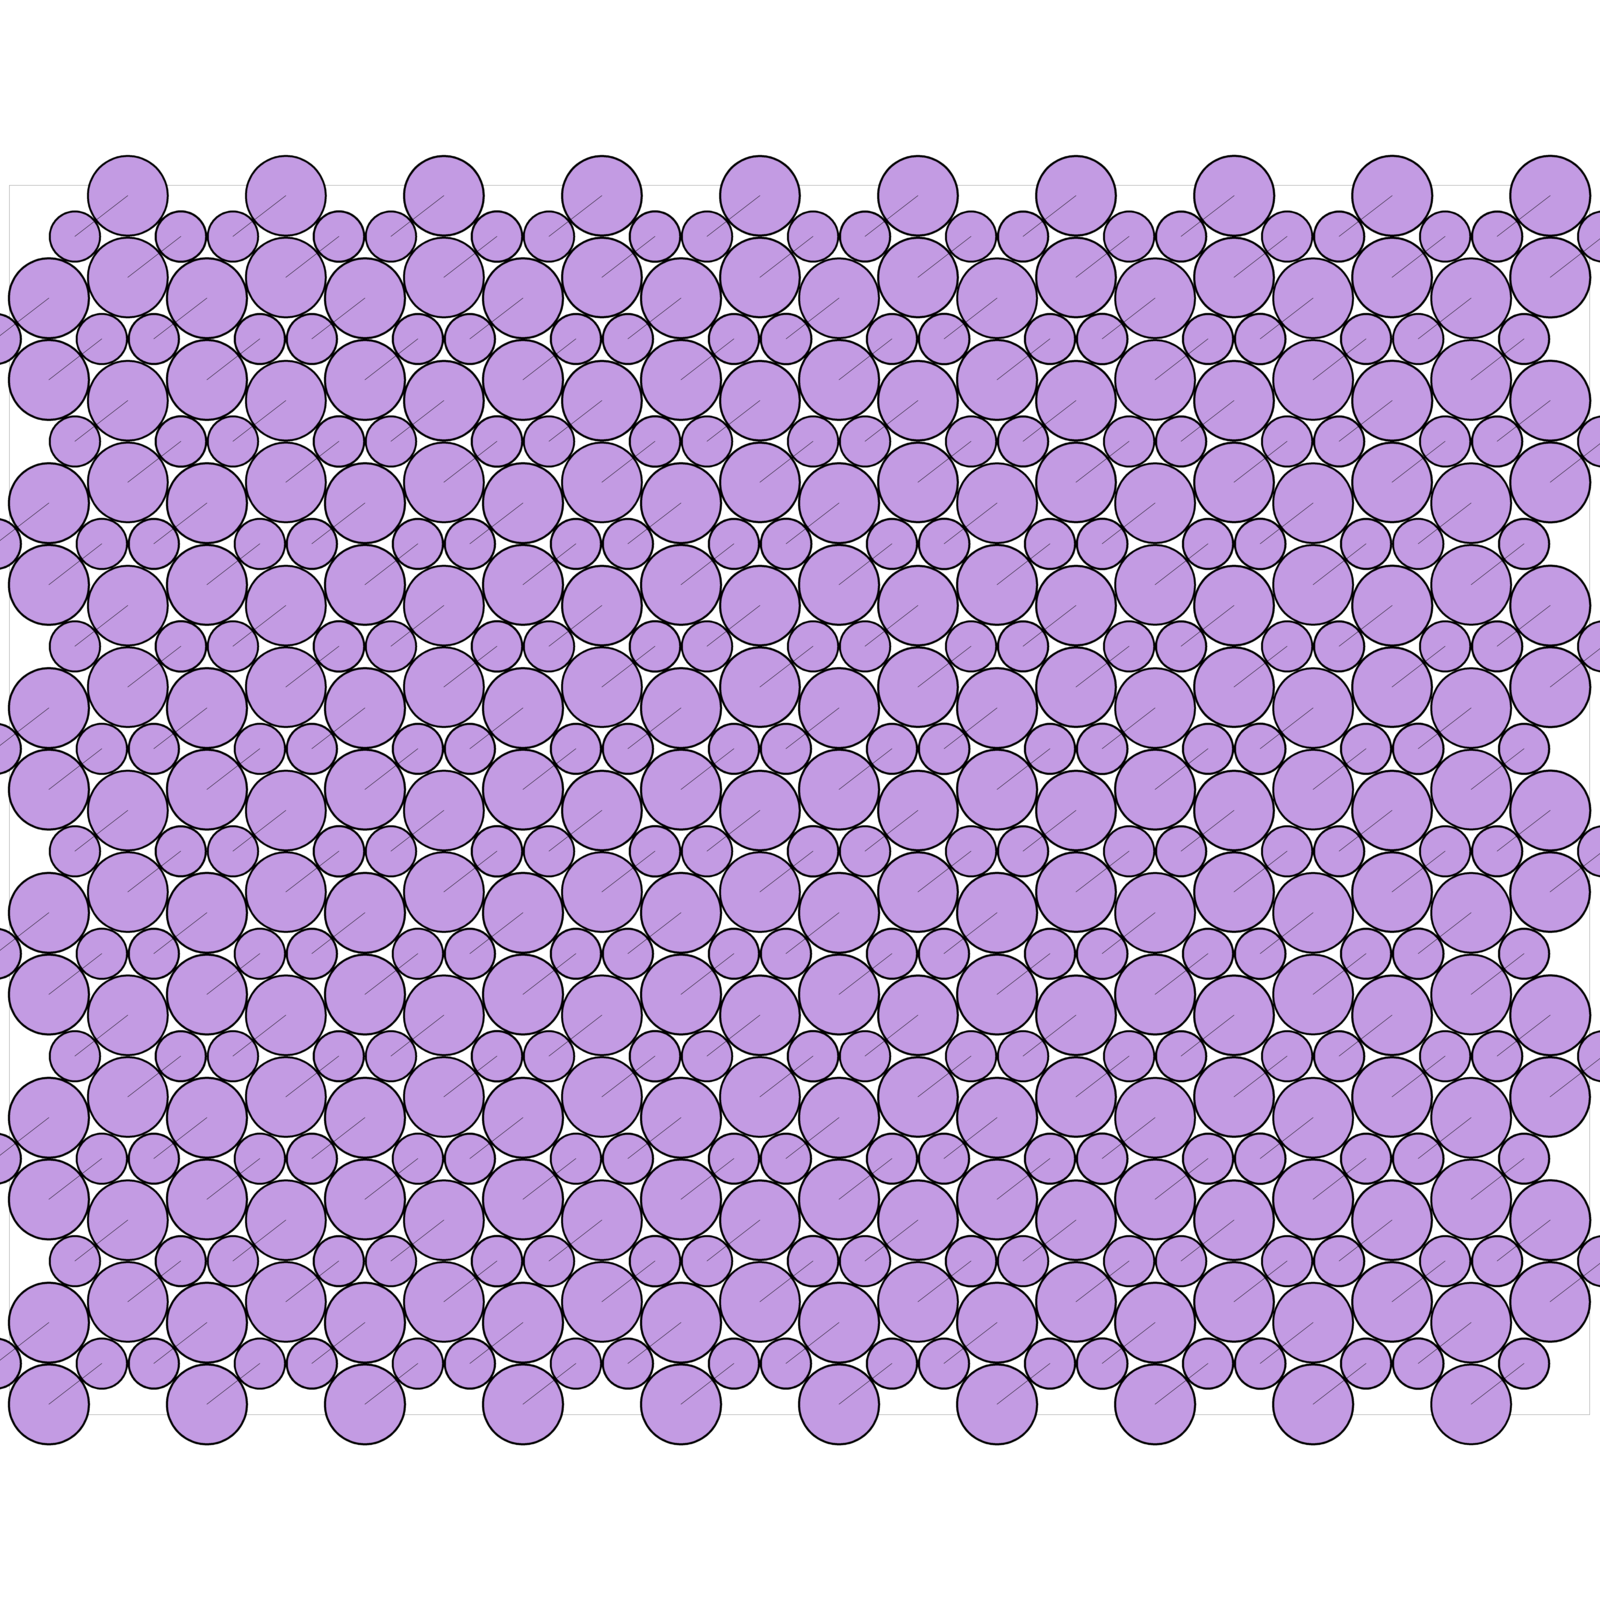
\includegraphics[width=\linewidth]{ordered-local}
        \caption{}
        \label{fig:orderd local}
    \end{subfigure}
    \caption{Comparison of the local order parameter on the ordered \subfigref{ordered local} and random \figref{random local} configurations of the \dcon molecule.}
    \label{fig:compact local}
\end{figure}

The crystalline structure of the \dcon molecule is defined by the underlying arrangement of particles, the arrangement of bonds on top of the arrangement of particles does not contribute to the crystal structure. As such we want an order parameter $O_\dcon$ based on the arrangement of individual particles rather than molecules. The way we have done this is to consider the local environment of each particle. In the crystalline structure each small particle has one small and four large neighbouring particles, and each large particle has three small and three large neighbours. By counting the number and type of neighbours particles with the appropriate local environment are classed as crystalline.

Using this targeted order parameter~\figref{compact frame} both the structures with random orientation and ordered orientation are completely crystalline. This demonstrates that the order parameters need to be carefully matched with the molecule to accurately identify the crystal phase.

\begin{figure}
    \begin{subfigure}[t]{0.5\linewidth}
        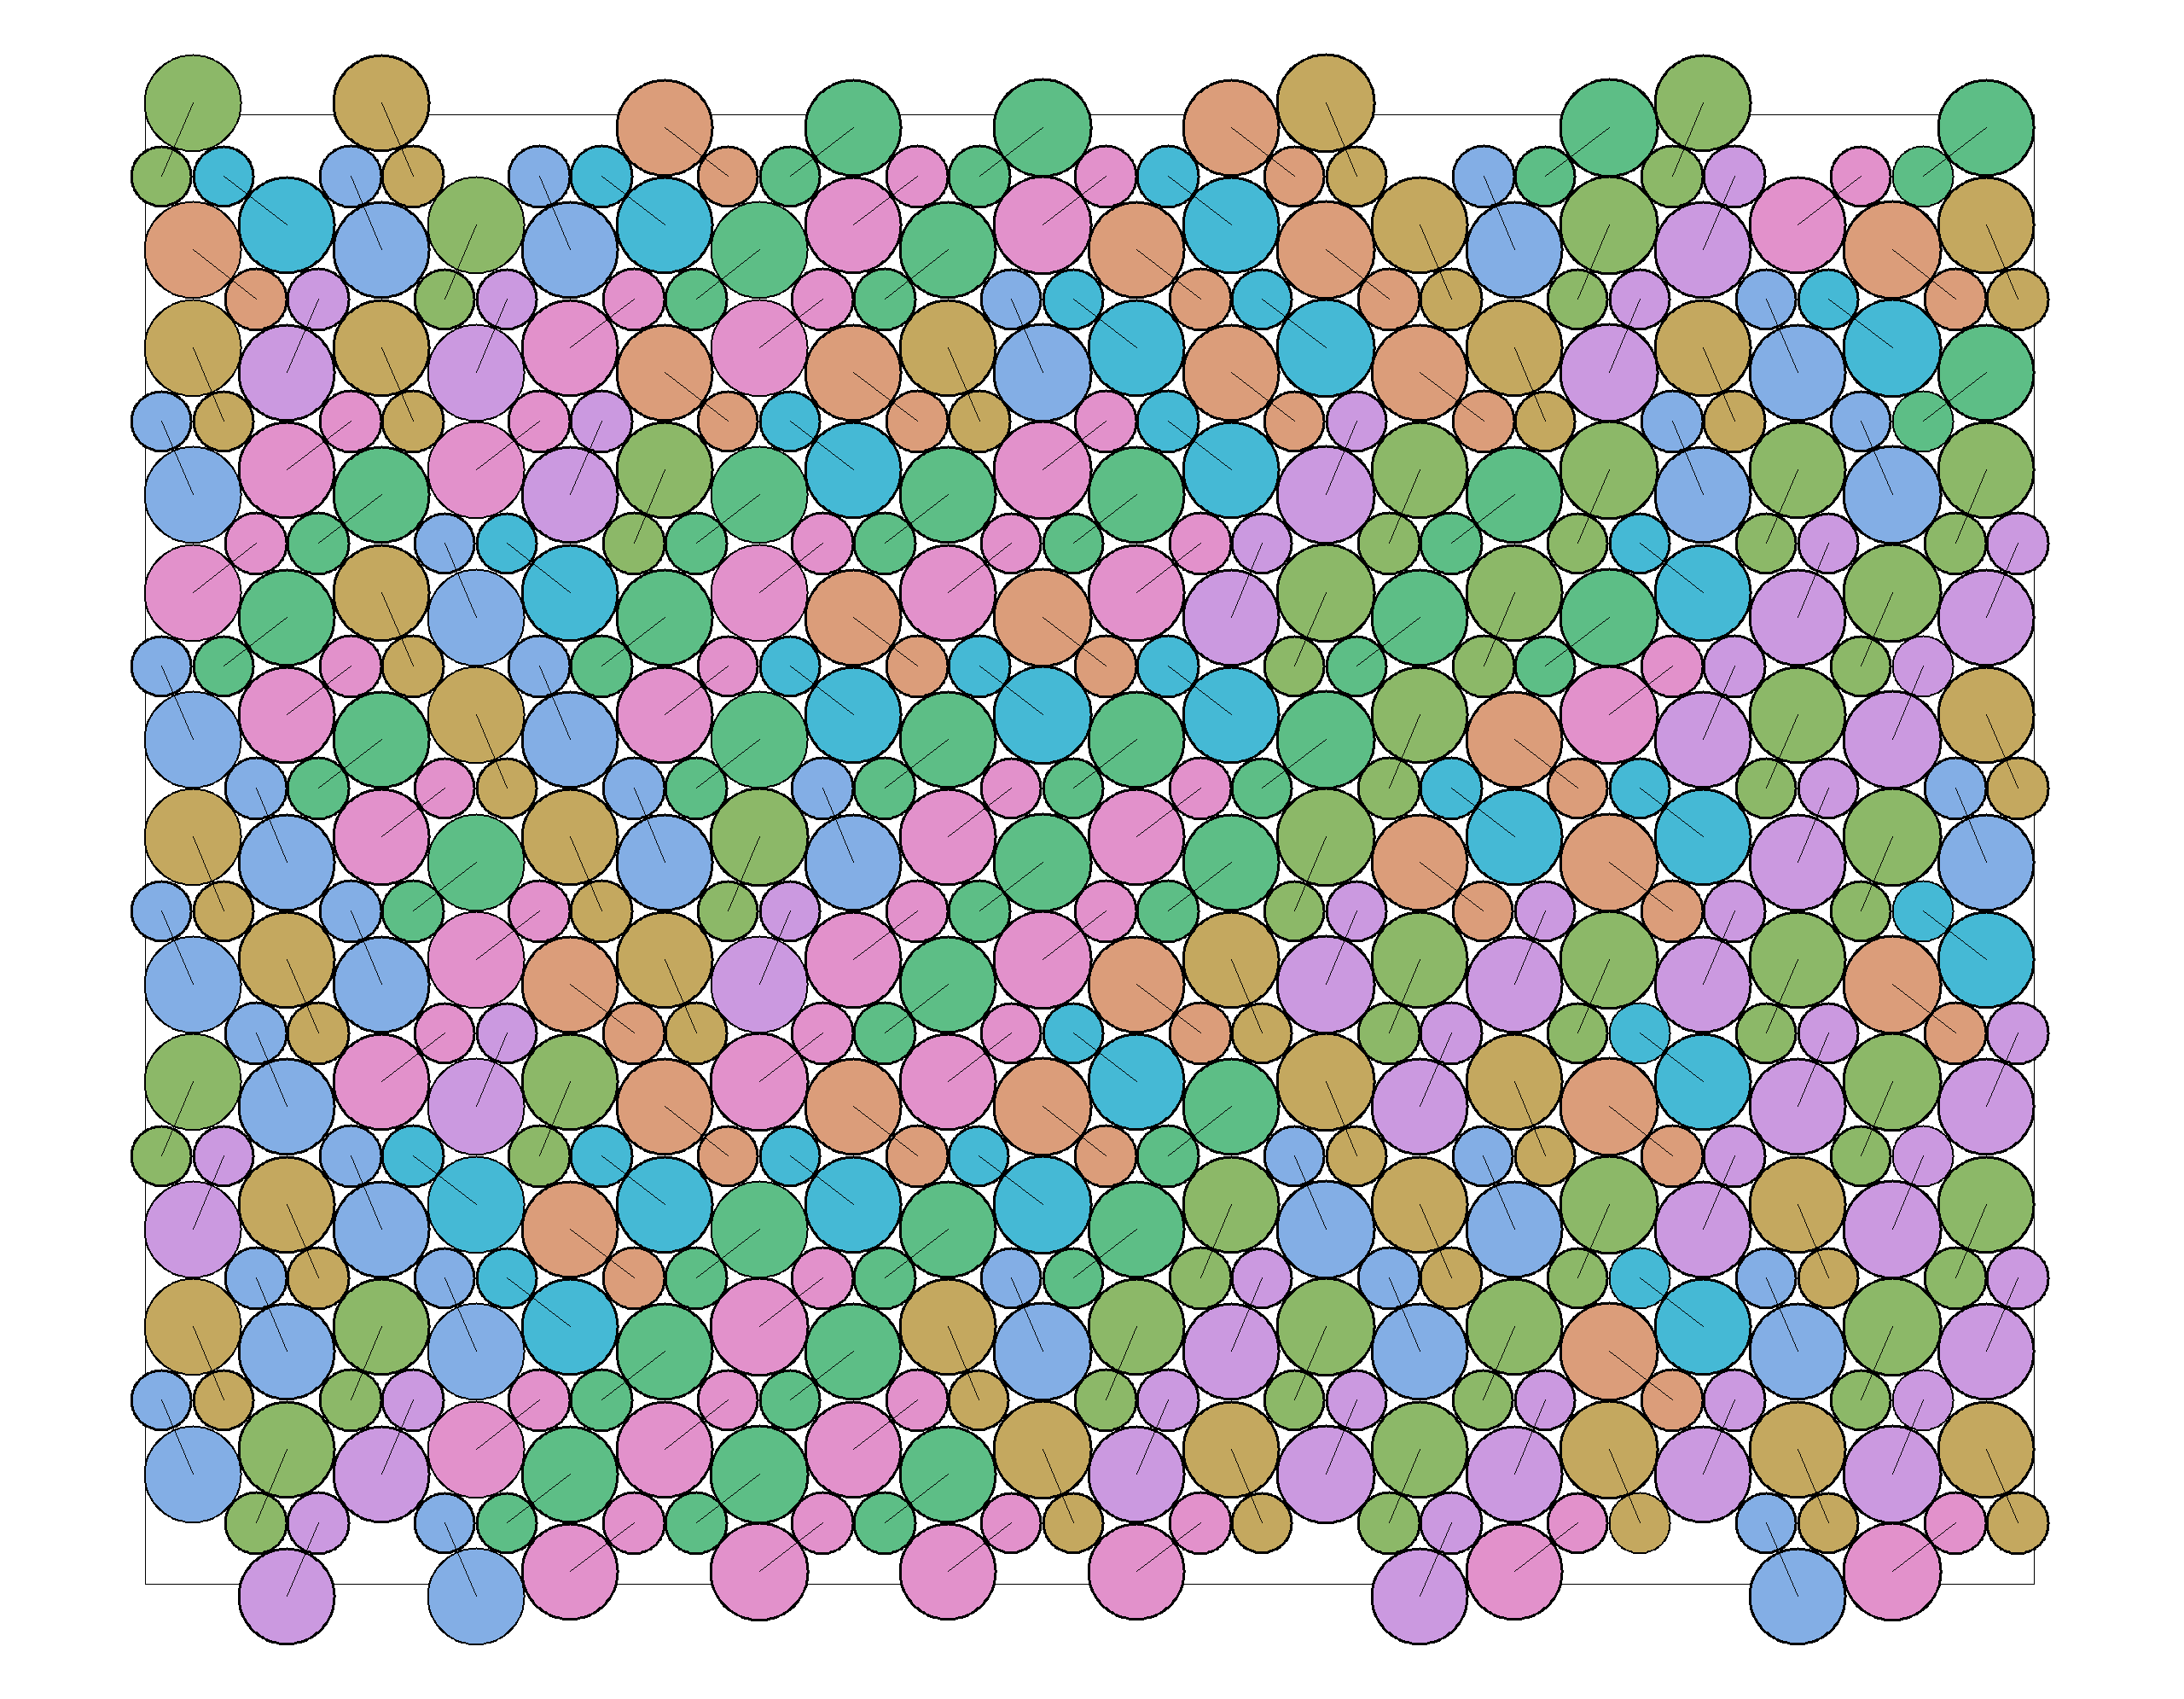
\includegraphics[width=\linewidth]{random-frame}
        \caption{}
        \label{fig:random frame}
    \end{subfigure}
    \begin{subfigure}[t]{0.5\linewidth}
        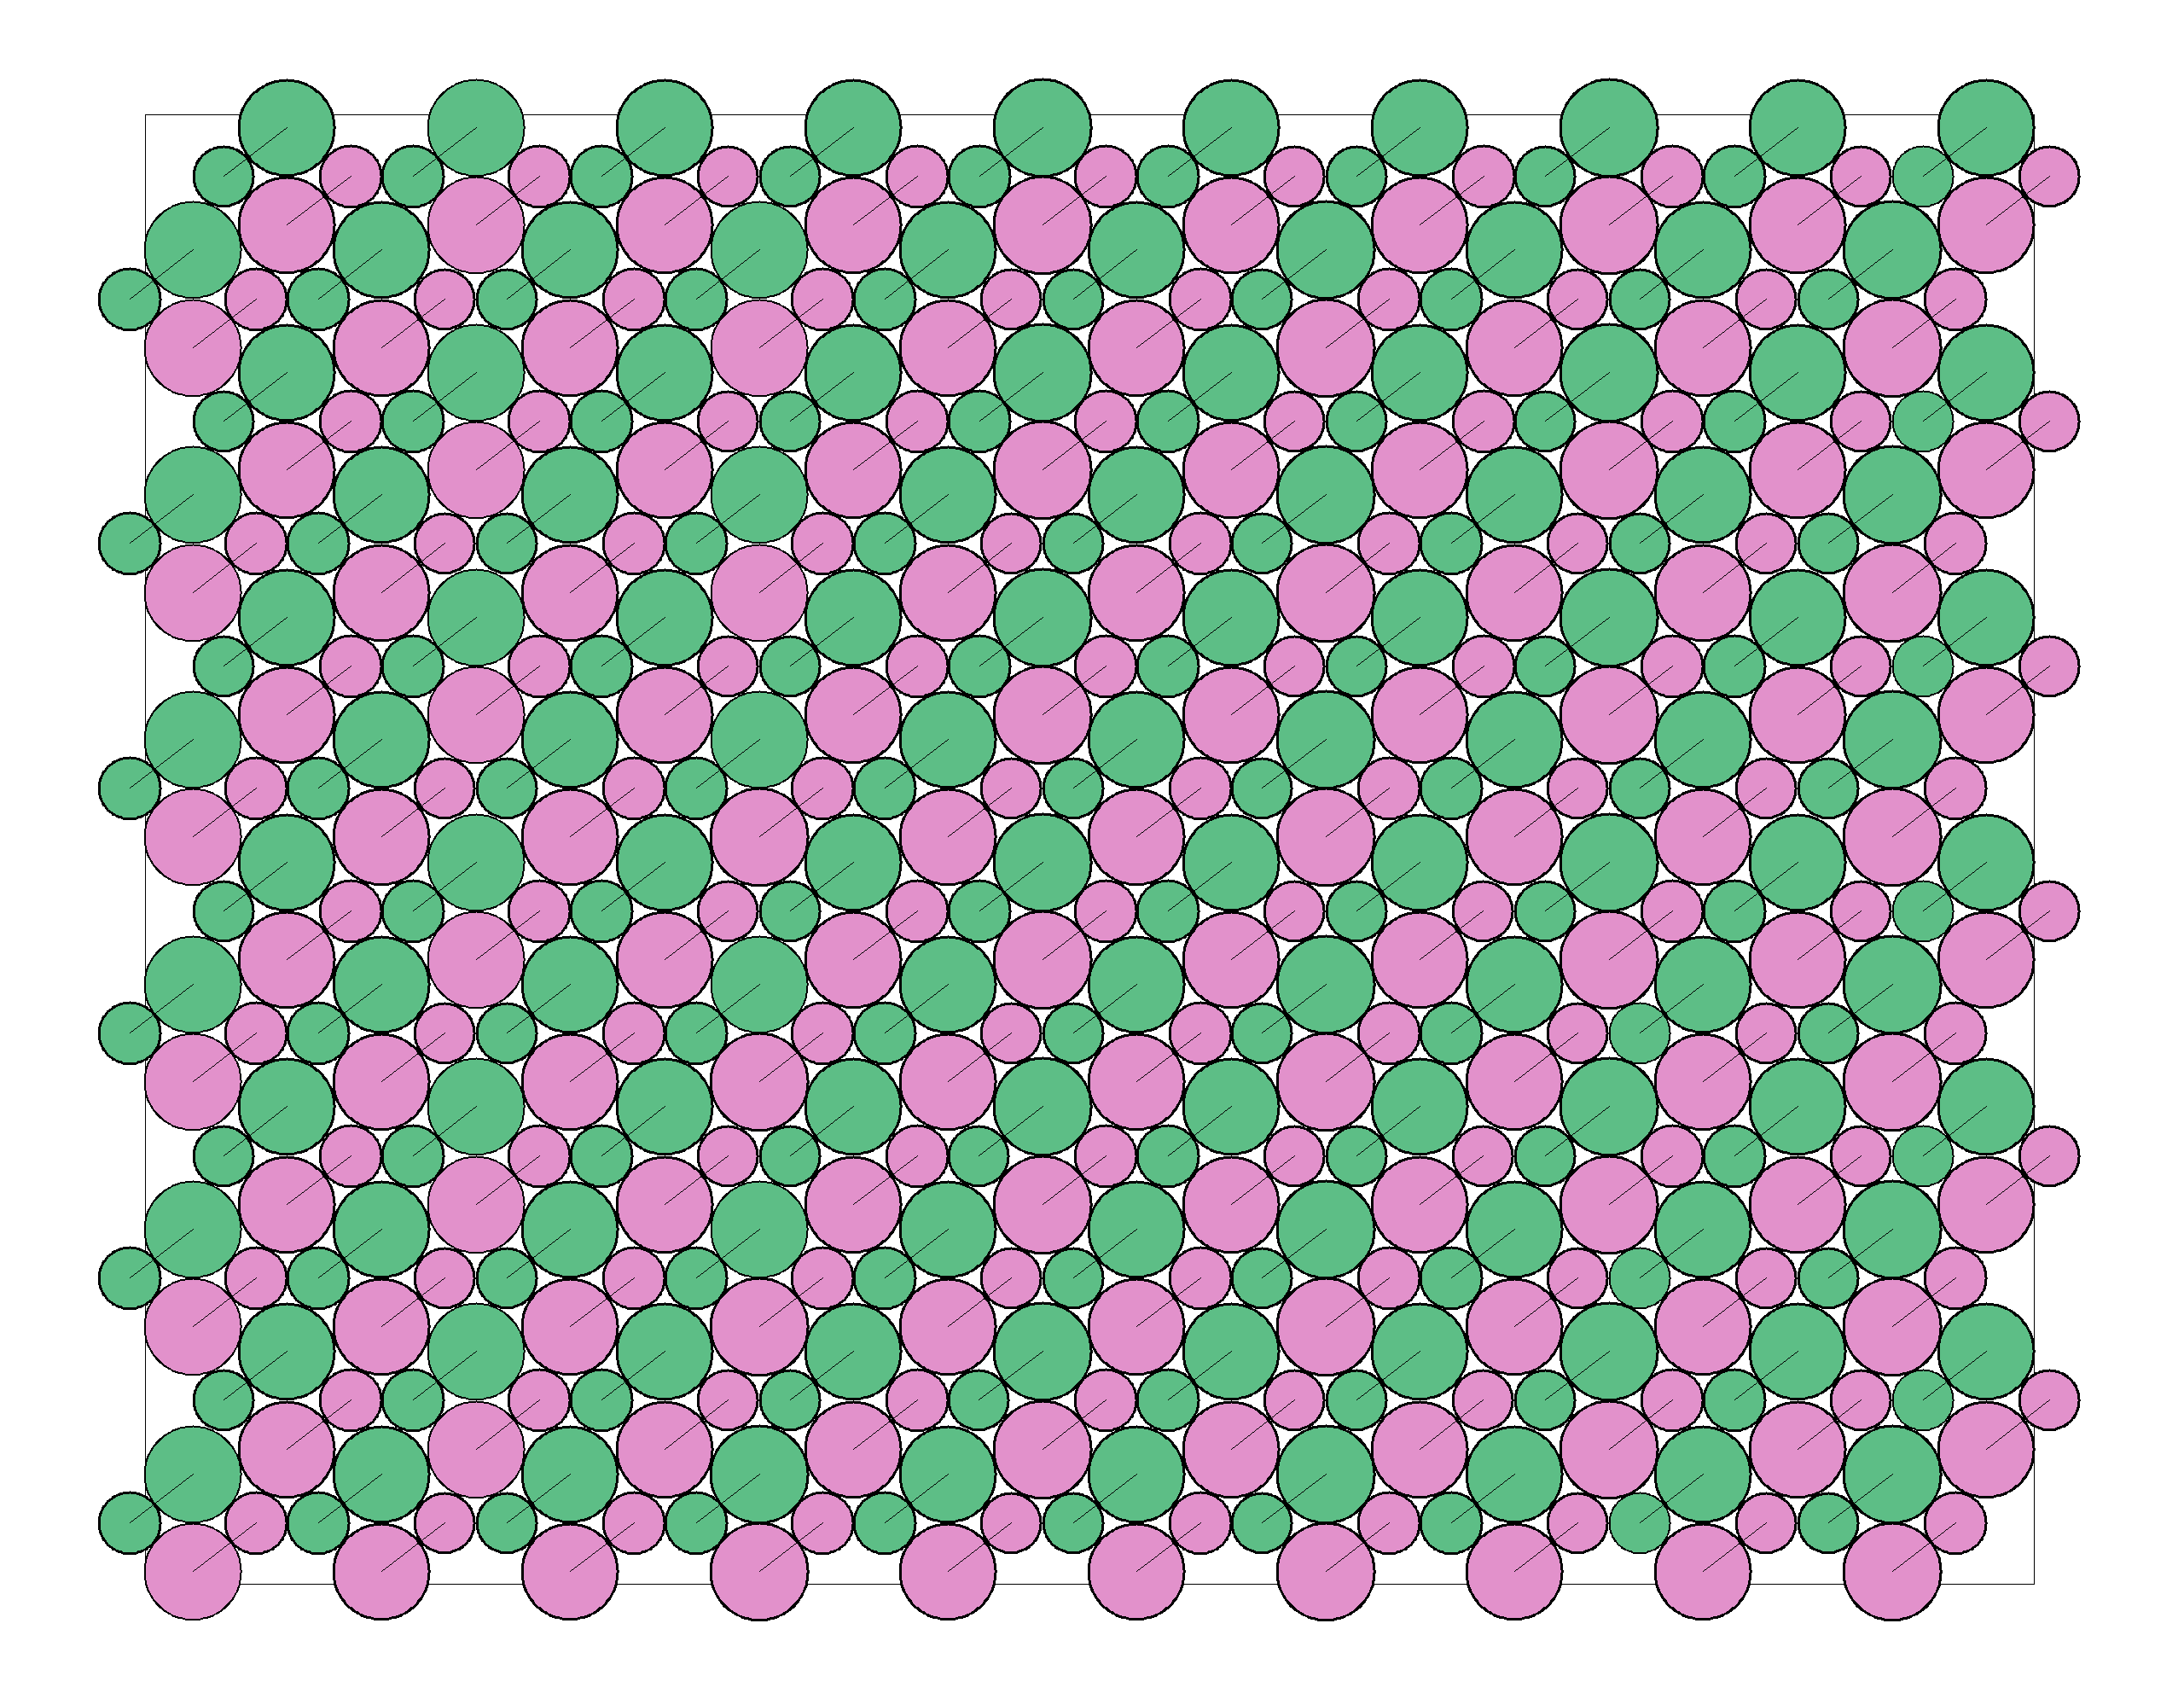
\includegraphics[width=\linewidth]{ordered-frame}
        \caption{}
        \label{fig:orderd frame}
    \end{subfigure}
    \caption{Comparison of the $O_\dcon$ order parameter on the ordered \subfigref{ordered local} and random \figref{random local} configurations of the \dcon molecule. Crystalline molecules are coloured according to their orientation and amorphous molecules are grey.}
    \label{fig:compact local}
\end{figure}

\section{The Structure in Amorphous Ground States}

While liquids show no long range anisotropy (i.e. they are isotropic) there is no reason why they might not accumulate short range structure as they are cooled below their freezing point. By \emph{short range} or \emph{local} structure we are referring to small clusters of particles that adopt an ordered arrangement that does not extend beyond the cluster. Using the tools developed above, in this section we investigate local structure of the supercooled liquid state.

The \done molecule~\figref{done order} shows a small degree of long range ordering in the radial distribution function which we can see as mostly small clusters of crystalline order, with some larger crystals in the local order parameter. These larger crystals are the crystal phase nucleating and their presence in the ground state structure suggests that it will be possible to grow crystals of the \done molecule in \textchapref{crystallisation}.

\begin{figure}
    \centering
    \begin{subfigure}[t]{0.45\linewidth}
        \includegraphics[width=\linewidth]{{{Snowman-0.80-0.637556-1.0-radial}}}
        \caption{}
        \label{fig:done radial}
    \end{subfigure}\hfill
    \begin{subfigure}[t]{0.45\linewidth}
        \includegraphics[width=\textwidth]{{{Snowman-0.80-0.637556-1.0-frame-0320000191}}}
        \caption{}
        \label{fig:done inherent}
    \end{subfigure}\hfill
    \caption{Radial distribution function \subfigref{done radial} and local ordering \subfigref{done inherent} of \done molecule. The broad peaks of the radial distribution function out a distance of 12 indicate some longer range ordering present in the structure which we see in the configuration as small clusters of crystalline ordering. The large cluster shows a nucleation event demonstrating that these events are possible.}
    \label{fig:done order}
\end{figure}

The ground state of the \dcon appears to be amorphous from the radial distribution function~\figref{dcon inherent} however from the local order parameter we see see regions of orientationally disordered crystalline order. In developing the local order parameter for \dcon we used the order of the particles as a measure of the order of the molecules, we can define a radial distribution function in the same way such that we are looking at the distances between each particle rather than each center of mass. This alternate radial distribution function gives \textfigref{dcon radial part} which shows long range ordering like we observe with the local order parameter.

\begin{figure}
    \centering
    \begin{subfigure}[t]{0.5\linewidth}
        \includegraphics[width=\linewidth]{{{Snowman-1.55-0.637556-1.637556-radial}}}
        \caption{}
        \label{fig:dcon radial}
    \end{subfigure}\hfill
    \begin{subfigure}[t]{0.5\linewidth}
        \includegraphics[width=\textwidth]{{{Snowman-1.55-0.637556-1.637556-frame-0320000182}}}
        \caption{}
        \label{fig:dcon inherent}
    \end{subfigure}
    \caption{Radial distribution function \subfigref{dcon radial} and local order parameter \subfigref{dcon inherent} of the \dcon molecule. The initial peaks of the radial distribution function are incredibly sharp showing strong short range ordering, however this order only extends to the second shell, this is contrasting with the local order parameter which shows clusters of orientationally disorderd crustal formation.}
        \label{fig:dcon order}
\end{figure}

\begin{figure}
    \centering
    \includegraphics[width=0.5\linewidth]{{{Snowman-1.55-0.637556-1.637556-radial_part}}}
    \caption{Radial particle distribution function for the \dcon molecule. This is a distribution of interparticle distances rather than center of mass distances. This figure shows the presence of medium range ordering in the peaks extending out to a distance of 12.}
    \label{fig:dcon radial part}
\end{figure}

The \tri molecule shows no ordering in liquid phase~\figref{tri order} from either the radial distribution function or the local order parameter. While there are some regions of local orientational order indicated by coloured molecules, these are a combination of the molecules occupying all the possible arrangements and false positives. From inspection the regions of local order identified are not representative of any longer range order. This is intriguing since the \tri molecule was taken further below the melting point than either of the other molecules with no indication of any order, a truly amorphous phase.

\begin{figure}
    \begin{subfigure}{0.5\linewidth}
        \includegraphics[width=\linewidth]{{{Trimer-1.05-0.637556-1.00-120-radial}}}
        \caption{}
        \label{fig:tri radial}
    \end{subfigure}
    \label{fig:radial distributions}
    \begin{subfigure}{0.5\linewidth}
        \includegraphics[width=\textwidth]{{{Trimer-1.00-0.637556-1.00-120-frame-0320000177}}}
        \caption{}
        \label{fig:tri inherent}
    \end{subfigure}
    \caption{Radial distribution function \subfigref{tri radial} and local order parameter \subfigref{tri inherent} of the \tri molecule. Neither the radial distribution function or the local order parameter display any signs of ordering, a truly amorphous phase.}
    \label{fig:tri order}
\end{figure}

\section{Summary}

In this Chapter we have identified the most stable crystal forms of each of our molecules as well as order parameters enabling us to distinguish the amorphous liquid phase from the ordered crystal phase. In investigating order in the \dcon molecule we identified that using a single order parameter for all molecules is inadequate and that the order parameters need to be targeted. The order parameters we have identified will allow us to investigate the growth of the crystal form the liquid phase in the next Chapter.
